% 04 — Zadatak 4: robusna stabilizacija prekidačkog (switching) sustava.

\section{Zadatak 4 --- robusna stabilizacija prekidačkog sustava}
\label{sec:zad4}

\subsection{Opis vremenski promjenjivog sustava}
\label{sec:zad4:opis}

Promatra se vremenski promjenjiv sustav \cite[str.~2]{jokic_zadatak}
\begin{equation}
  \dot{x}(t) = A(t)\,x(t) + B\,u(t), \qquad
  A(t) = \begin{cases}
    A_{\text{parno}}, & \lfloor t \rfloor \text{ paran},\\
    A_{\text{neparno}}, & \lfloor t \rfloor \text{ neparan},
  \end{cases}
  \label{eq:z4sys}
\end{equation}
uz
\begin{equation}
  A_{\text{parno}} = \begin{bmatrix} -1 & -\tfrac{1}{6}\pi \\[2pt] \tfrac{3}{2}\pi & -1 \end{bmatrix}, \qquad
  A_{\text{neparno}} = \begin{bmatrix} -1 & -\tfrac{3}{2}\pi \\[2pt] \tfrac{1}{6}\pi & -1 \end{bmatrix}.
\end{equation}
Riječ je o hibridnom sustavu sa skokovitom promjenom dinamike u cjelobrojnim
trenucima; između dva prekapčanja sustav je linearan i vremenski invarijantan.

\subsection{Stabilnost pojedinih dinamičkih modova}
\label{sec:zad4:modovi}

Za matricu oblika $\left[\begin{smallmatrix} -1 & -\alpha \\ \beta & -1 \end{smallmatrix}\right]$
karakteristični polinom je $(\lambda+1)^2 + \alpha\beta = 0$, pa je
$\lambda = -1 \pm \mathrm{i}\sqrt{\alpha\beta}$. U oba moda umnožak
izvandijagonalnih elemenata je jednak,
\begin{equation}
  \alpha\beta = \frac{\pi}{6}\cdot\frac{3\pi}{2} = \frac{\pi^2}{4},
\end{equation}
pa oba moda imaju iste svojstvene vrijednosti
\begin{equation}
  \lambda_{1,2} = -1 \pm \mathrm{i}\,\frac{\pi}{2} .
\end{equation}
Realni dio je $-1 < 0$, dakle \textbf{obje su matrice Hurwitzove} i oba su
dinamička moda asimptotski stabilna \cite[str.~5]{jokic_ljapunov}.

\subsection{Simulacija sustava u otvorenom krugu}
\label{sec:zad4:simulacija}

Stabilnost pojedinih modova \emph{ne} povlači stabilnost prekidačkog sustava.
Kako je prekapčanje periodično s periodom $2$ (jedna sekunda u svakom modu),
stabilnost se ispituje monodromijskom matricom preko jednog perioda:
\begin{equation}
  \Phi = e^{A_{\text{neparno}}\cdot 1}\,e^{A_{\text{parno}}\cdot 1} .
\end{equation}
Sustav je stabilan ako i samo ako je spektralni radijus $\rho(\Phi) < 1$.
Izračun daje
\begin{equation}
  \operatorname{eig}(\Phi) = \{-1{,}218018,\; -0{,}015037\}, \qquad
  \rho(\Phi) = 1{,}218018 > 1 ,
\end{equation}
pa je prekidački sustav \textbf{nestabilan}. Floquetov eksponent je
$\tfrac{1}{2}\ln\rho = +0{,}098612$, dakle amplituda raste kao $e^{0{,}0986\,t}$.

Gornji lijevi i desni dio slike~\ref{fig:z4} potvrđuju zaključak: uz
$x(0) = (1,0)^{\mathsf T}$ stanja osciliraju s rastućom amplitudom, a trajektorija
se u prostoru stanja spiralno udaljava od ishodišta.

Objašnjenje je geometrijsko. Svaki mod sam za sebe rotira trajektoriju prema
ishodištu, ali dva moda rotiraju u različitim "smjerovima rastezanja". Prekapčanje
je vremenski usklađeno tako da svaki mod preuzme stanje u trenutku kad ga može
pojačati; energija koju jedan mod ukloni, drugi doda s viškom. Zato provjera
svojstvenih vrijednosti pojedinih modova nije dovoljna za prekidačke sustave.

\subsection{Sinteza statičkog regulatora}
\label{sec:zad4:regulator}

Uz $B = (1,0)^{\mathsf T}$ traži se statički regulator $u = Kx$ takav da je
zatvoreni krug $\dot{x} = (A(t) + BK)x$ eksponencijalno stabilan.

Dovoljan uvjet je postojanje \emph{zajedničke} kvadratne Ljapunovljeve funkcije
$V(x) = x^{\mathsf T}Px$, $P \succ 0$, za koju $\dot V < 0$ u oba moda
\cite[str.~4]{jokic_ljapunov}:
\begin{equation}
  (A_i + BK)^{\mathsf T}P + P(A_i + BK) \prec 0, \qquad i \in \{\text{parno}, \text{neparno}\} .
  \label{eq:z4lmi}
\end{equation}
Postoji li takav par $(P,K)$, zatvoreni krug je eksponencijalno stabilan za
\emph{proizvoljno} prekapčanje, ne samo za ovo periodično --- a to je jače od
onoga što zadatak traži.

Uvjet \eqref{eq:z4lmi} je bilinearan u $(P,K)$, no supstitucijom $Q = P^{-1}$ i
$Y = KQ$ prelazi u linearne matrične nejednakosti
\begin{equation}
  A_iQ + QA_i^{\mathsf T} + BY + Y^{\mathsf T}B^{\mathsf T} \prec 0, \quad Q \succ 0,
  \qquad K = YQ^{-1},
  \label{eq:z4lmi2}
\end{equation}
što je standardni put preko semidefinitnog programiranja \cite[str.~23]{jokic_qcpsdp}.
Na korištenom sustavu nije bio instaliran SDP rješavač, pa je certifikat izveden
analitički --- za sustav drugog reda to je izvedivo u zatvorenoj formi.

Uz $P = I$ i $K = [\,k_1\;\; k_2\,]$ zatvoreni krug ima oblik
$A_i + BK = \left[\begin{smallmatrix} -1+k_1 & c_i \\ \beta_i & -1 \end{smallmatrix}\right]$,
gdje je $c_{\text{parno}} = k_2 - \pi/6$, $\beta_{\text{parno}} = 3\pi/2$ te
$c_{\text{neparno}} = k_2 - 3\pi/2$, $\beta_{\text{neparno}} = \pi/6$. Tada je
\begin{equation}
  (A_i+BK)^{\mathsf T} + (A_i+BK) =
  \begin{bmatrix} 2(-1+k_1) & c_i + \beta_i \\ c_i + \beta_i & -2 \end{bmatrix} .
\end{equation}
Izbor
\begin{equation}
  k_2 = -\frac{4\pi}{3}
\end{equation}
poništava izvandijagonalni član parnog moda, pa on postaje dijagonalan i
negativno definitan čim je $k_1 < 1$. Za neparni mod uvjet negativne
definitnosti (pozitivna determinanta uz negativan trag) daje
\begin{equation}
  -4(-1+k_1) > \left(c_{\text{neparno}} + \beta_{\text{neparno}}\right)^2
  \quad\Longrightarrow\quad
  k_1 < 1 - \frac{16\pi^2}{9} = -16{,}545963 .
  \label{eq:z4bound}
\end{equation}

Odabrano je
\begin{equation}
  \boxed{\;K = \left[\,-20 \quad -\tfrac{4\pi}{3}\,\right] = [\,-20 \quad -4{,}188790\,].\;}
\end{equation}

Numerička provjera potvrđuje granicu \eqref{eq:z4bound}: za $k_1 = -16{,}6$ uvjet
je zadovoljen, a za $k_1 = -16{,}5$ nije. Uz odabrani $K$ i $P = I$ dobiva se

\begin{table}[htbp]
  \centering
  \caption{Certifikat stabilnosti zatvorenog kruga uz $P = I$.}
  \label{tab:z4}
  \begin{tabular}{lcc}
    \hline
    Mod & $\operatorname{eig}(A_i + BK)$ & $\operatorname{eig}\!\big((A_i+BK)^{\mathsf T}P + P(A_i+BK)\big)$ \\
    \hline
    parno    & $-19{,}820,\; -2{,}180$ & $-42{,}000,\; -2{,}000$ \\
    neparno  & $-20{,}764,\; -1{,}236$ & $-43{,}684,\; -0{,}316$ \\
    \hline
  \end{tabular}
\end{table}

Obje su matrice negativno definitne, čime je \eqref{eq:z4lmi} zadovoljen.
Iz $\dot V \le -0{,}3163\,V$ slijedi eksponencijalna ocjena
\begin{equation}
  \lVert x(t)\rVert \le \lVert x(0)\rVert\, e^{-0{,}1581\,t} .
\end{equation}

\subsection{Simulacija zatvorenog kruga}
\label{sec:zad4:zatvoreni}

Spektralni radijus monodromijske matrice zatvorenog kruga iznosi
$\rho(\Phi_{\text{cl}}) = 3{,}126\cdot10^{-2} \ll 1$, dakle amplituda se po
periodu smanji približno tridesetak puta. Donji dio slike~\ref{fig:z4} prikazuje
odziv uz isti početni uvjet $x(0) = (1,0)^{\mathsf T}$: stanja se ugase unutar
otprilike dvije sekunde, a trajektorija monotono ulazi u ishodište bez
oscilacija koje su obilježavale otvoreni krug.

\begin{figure}[htbp]
  \centering
  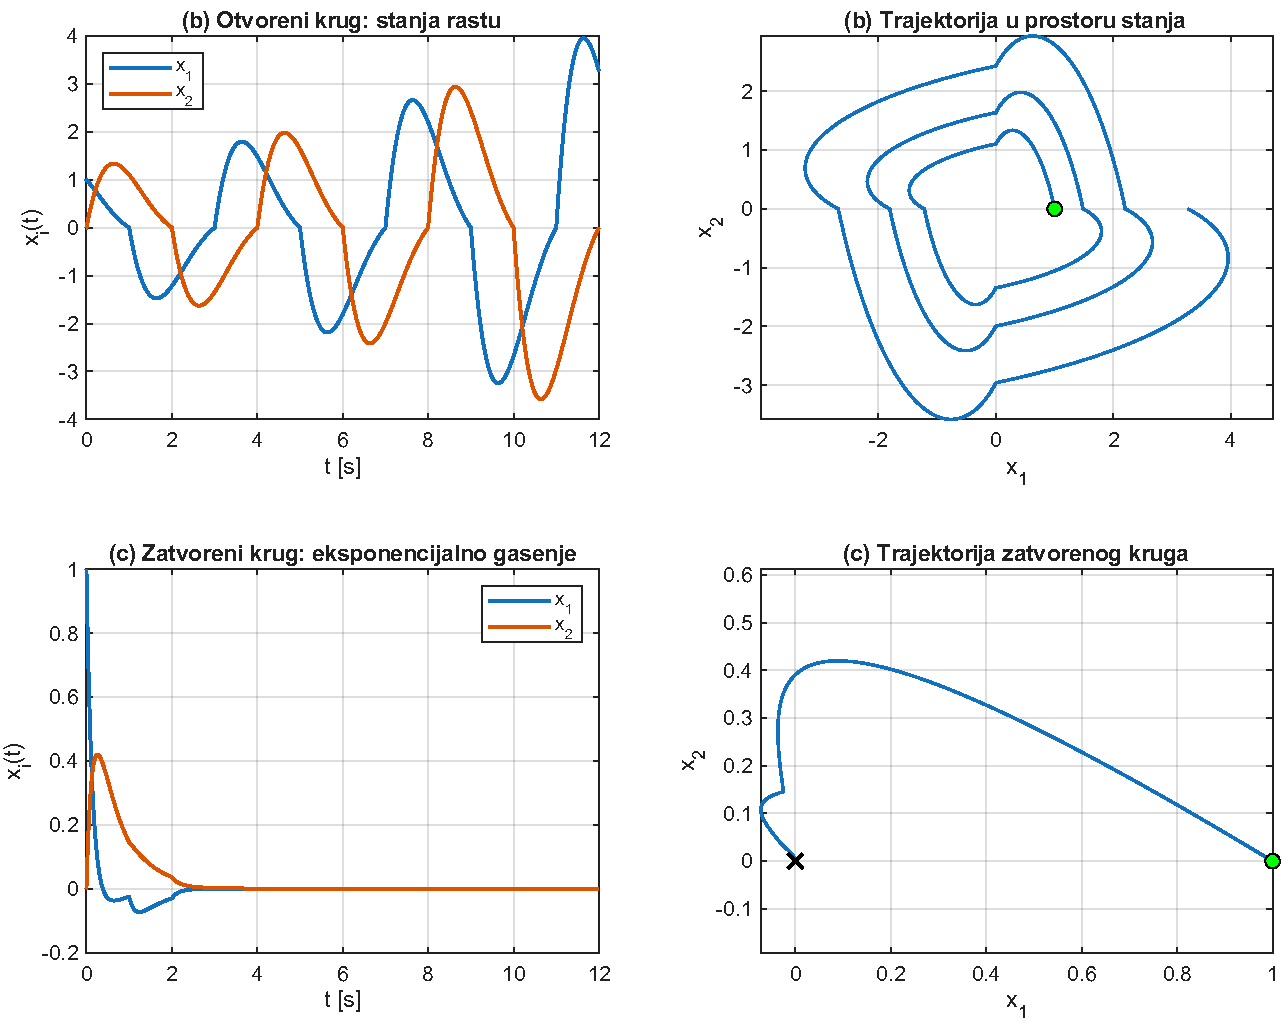
\includegraphics[width=\textwidth]{figures/zad4_switching.pdf}
  \caption{Prekidački sustav uz $x(0)=(1,0)^{\mathsf T}$. Gore: otvoreni krug ---
  stanja i trajektorija rastu unatoč tome što su oba moda Hurwitzova. Dolje:
  zatvoreni krug uz $u = Kx$ --- eksponencijalno gašenje.}
  \label{fig:z4}
\end{figure}

\subsection{Diskusija rezultata}
\label{sec:zad4:diskusija}

Zadatak dobro ilustrira tri stvari. Prvo, stabilnost svih pojedinačnih modova
nije dovoljna za stabilnost prekidačkog sustava --- ovdje su oba moda imala
identične svojstvene vrijednosti $-1 \pm \mathrm{i}\pi/2$, a sustav je ipak rastao
kao $e^{0{,}0986t}$. Drugo, ispravan alat je zajednička Ljapunovljeva funkcija:
ona daje certifikat neovisan o zakonu prekapčanja, dok analiza monodromijske
matrice vrijedi samo za točno ovaj periodični raspored. Treće, sinteza
regulatora prirodno se zapisuje kao LMI problem, čime ulazi u domenu
semidefinitnog programiranja i time u istu konveksnu okosnicu kao i prethodni
zadaci.

Cijena dobivenog rješenja je relativno velik pojačanje $k_1 = -20$. Uvjet
\eqref{eq:z4bound} pokazuje da je to nužno uz izbor $P = I$: granica
$1 - 16\pi^2/9 \approx -16{,}55$ posljedica je velikog raspona izvandijagonalnih
elemenata. Traženjem općenitijeg $P$ preko SDP-a mogao bi se dobiti manji
zahtjev na pojačanje, što je prirodan sljedeći korak ako bi upravljački signal
bio ograničen.
